\section*{CHƯƠNG 3. THIẾT KẾ HỆ THỐNG}
    \addcontentsline{toc}{section}{\numberline{}CHƯƠNG 3. THIẾT KẾ HỆ THỐNG}
    
\setcounter{section}{3}
    \setcounter{subsection}{0}
        \setcounter{figure}{0}
            \setcounter{table}{0}
%%-------------------------------------------------------%%
% --------------------------------------------------------%
%---------------------------------------------------------%

\subsection{Phân tích yêu cầu hệ thống}


\begin{figure}[!ht]
    \centering
    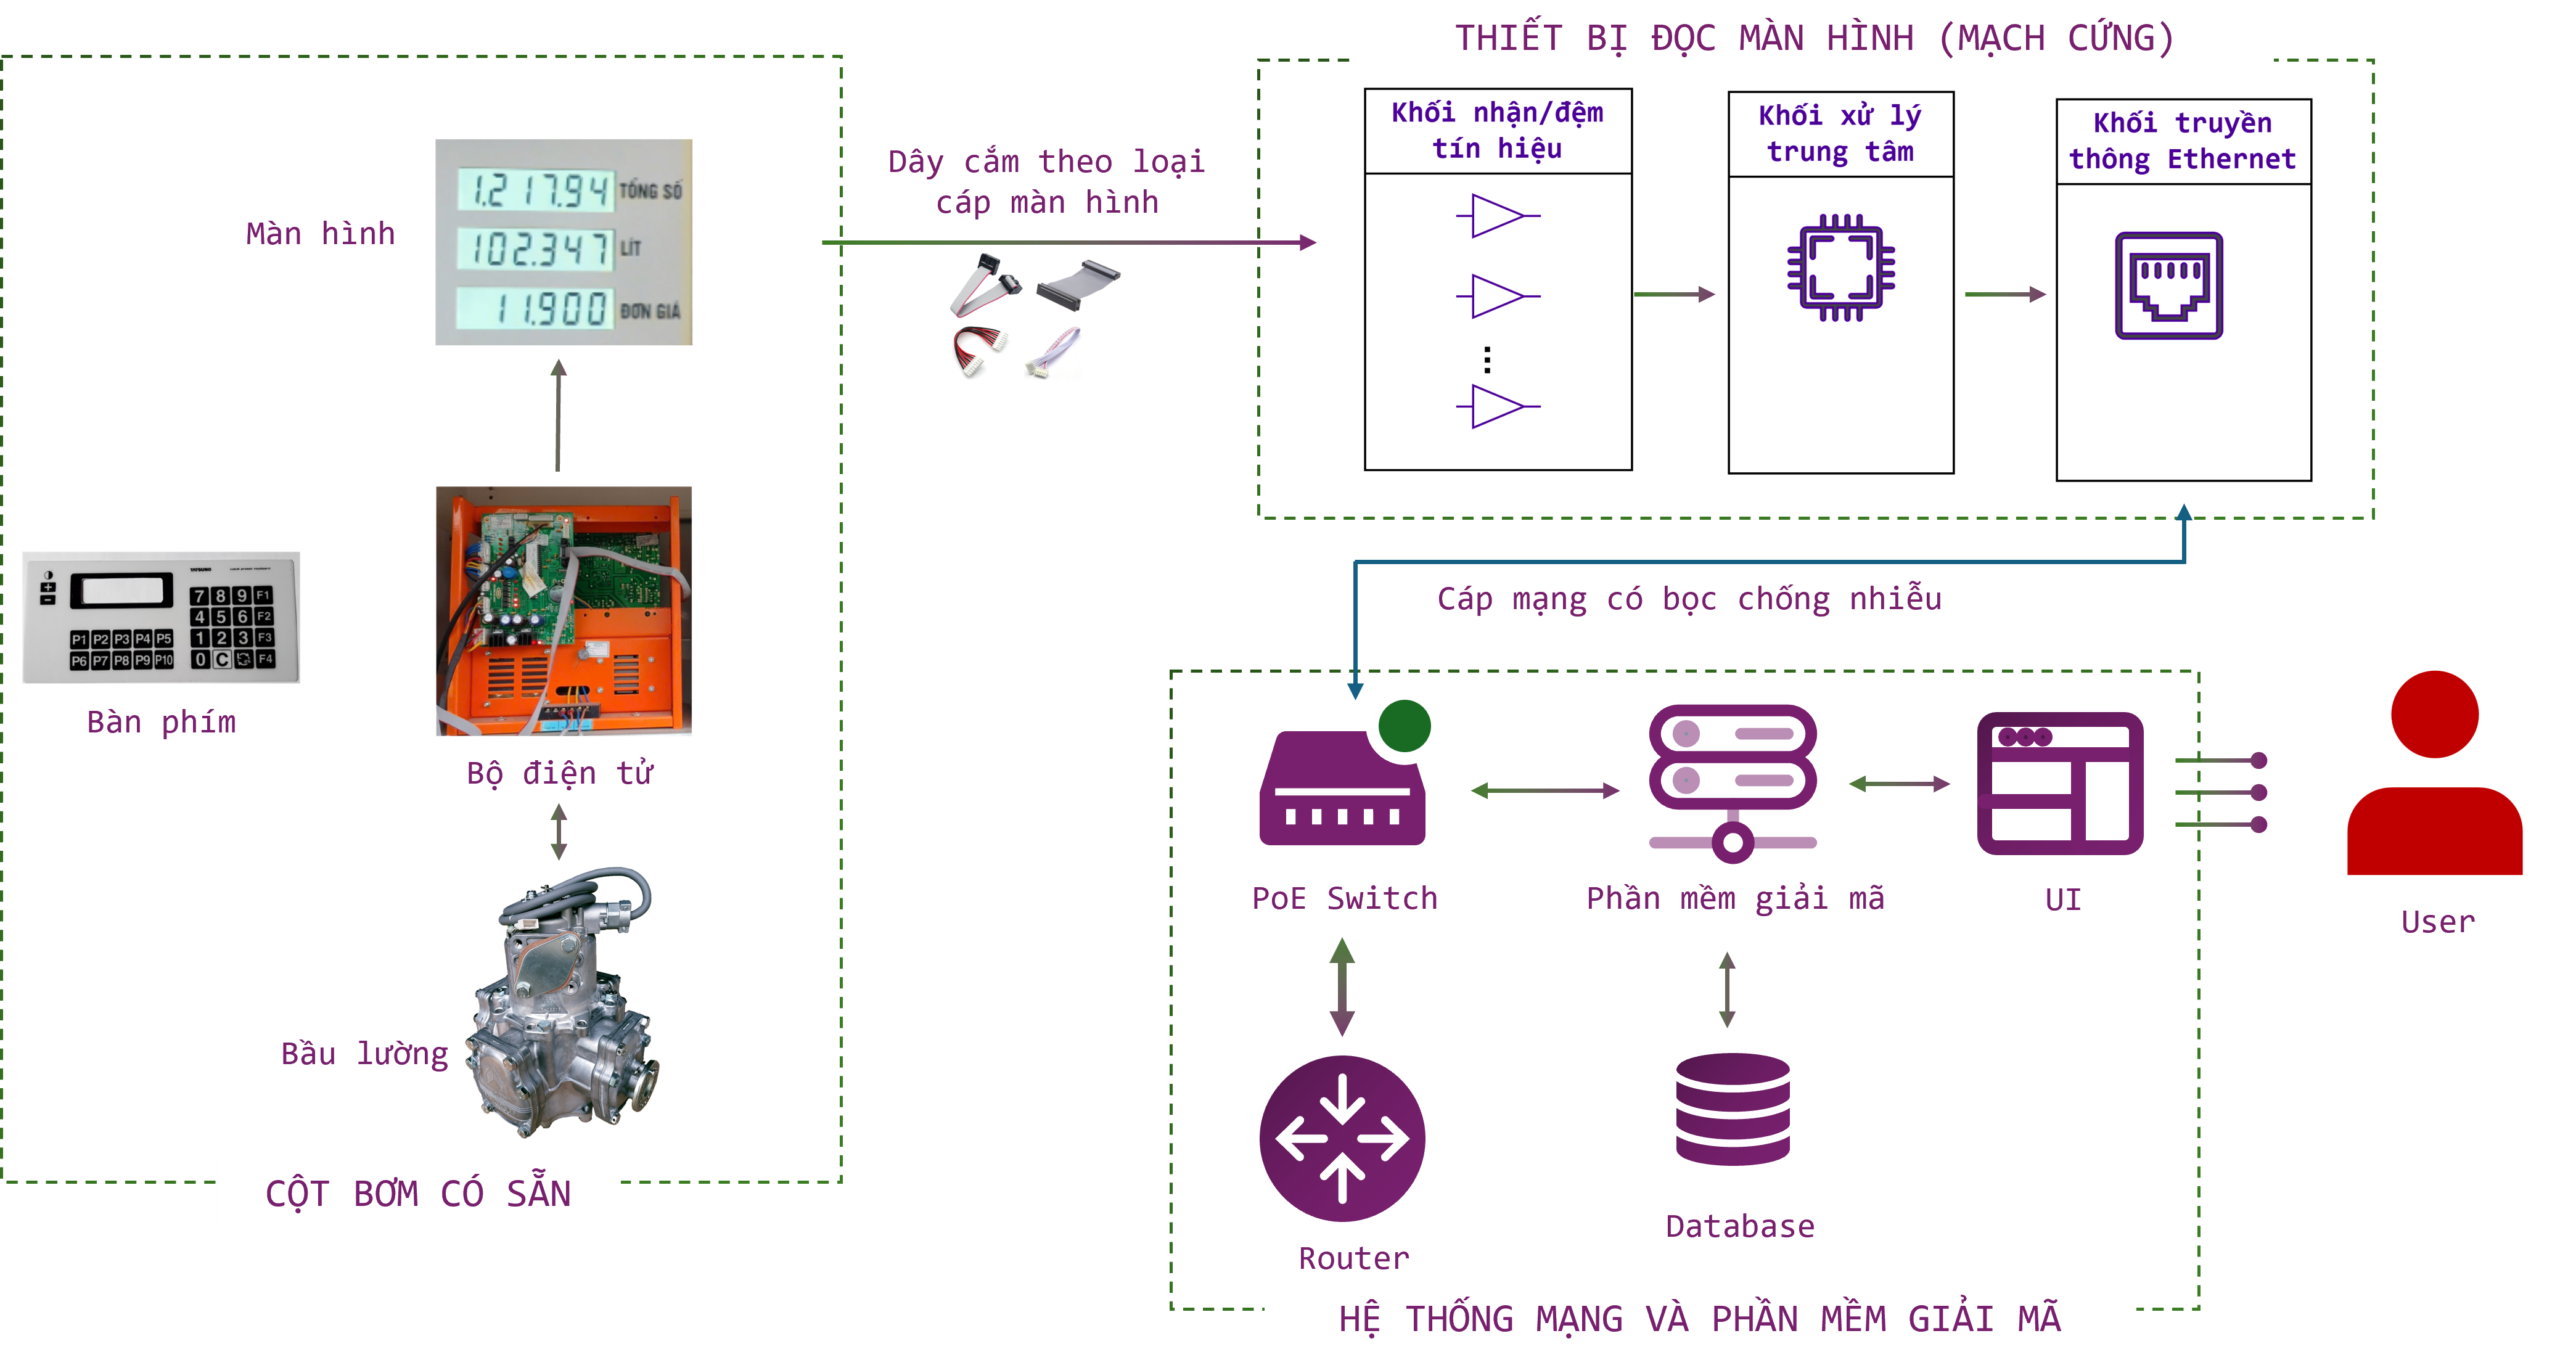
\includegraphics[width=1.0\linewidth]{Figures/Chap3_FunctionBlock-implementation.png}
    \caption{Các thành phần của hệ thống}
    \label{fig:hinh3.1}
\end{figure}

Các thành phần chính của hệ thống bao gồm:

\subsubsection{Thiết bị đọc ghi màn hình}


\hspace{0.8cm} Là mạch cứng gắn vào màn hình cột bơm, thu dữ liệu thô màn hình:
\begin{itemize}
   
    \item Kích cỡ: vừa, có thể lắp đặt trong cột bơm
    \item Tần số lấy mẫu: 100Hz
    \item Cấp nguồn riêng
    \item Nguồn và tín hiệu vào được cách ly quang, đảm bảo không có tín hiệu quay ngược trở lại màn hình
    \item Có 2 relay đóng ngắt có thể nối nối tiếp với cột bơm
    \item Giao tiếp, gửi dữ liệu thông qua Ethernet
    \item (Optional) Đầu vào tín hiệu (cáp và bộ chuyển đổi tín hiệu) có thể thích hợp với nhiều loại màn hình khác ngoài ZCheng để phục vụ thu thập và phân tích thêm các loại cột bơm khác.
    
\end{itemize}



\subsubsection{Phần mềm giải mã}

\hspace{0.8cm} Phần mềm giải mã đặt trong máy tính nội bộ tại trạm:

\begin{itemize}
    \item Đọc và giải mã tín hiệu tới màn hình với tần số 100Hz.
    \item Giao diện phần mềm hiển thị màn hình đã giải mã theo thời gian thực
    \item Phát hiện, lưu trữ các phiên bơm. Giao diện hiển thị các phiên bơm đã lưu trữ.
    \item Điều khiển đóng ngắt relay.
    \item Có cơ chế cập nhật firmware (OTA) cho thiết bị.    
\end{itemize}

\subsubsection{Hệ thống mạng}

\begin{itemize}
    \item POE Switch cấp nguồn riêng cho thiết bị đọc ghi màn hình
    \item Router điều khiển mạng LAN, cấp phát IP cho thiết bị
    \item Các thiết bị (thiết bị đọc ghi màn hình và phần mềm giải mã trong máy tính nội bộ) có thể tự động dò tìm và kết nối với nhau.
\end{itemize}

\subsection{Mô hình thiết kế tổng thể}

\hspace{0.8cm} Phần này nêu ra sơ đồ khối chức năng các thành phần hệ thống. Qua đó mô tả chức năng cụ thể của thành phần thông qua các khối, đồng thời mô tả cách các khối giao tiếp với nhau.

\subsubsection{Sơ đồ khối chức năng thiết bị đọc ghi màn hình (Device)}

\begin{figure}[!ht]
    \centering
    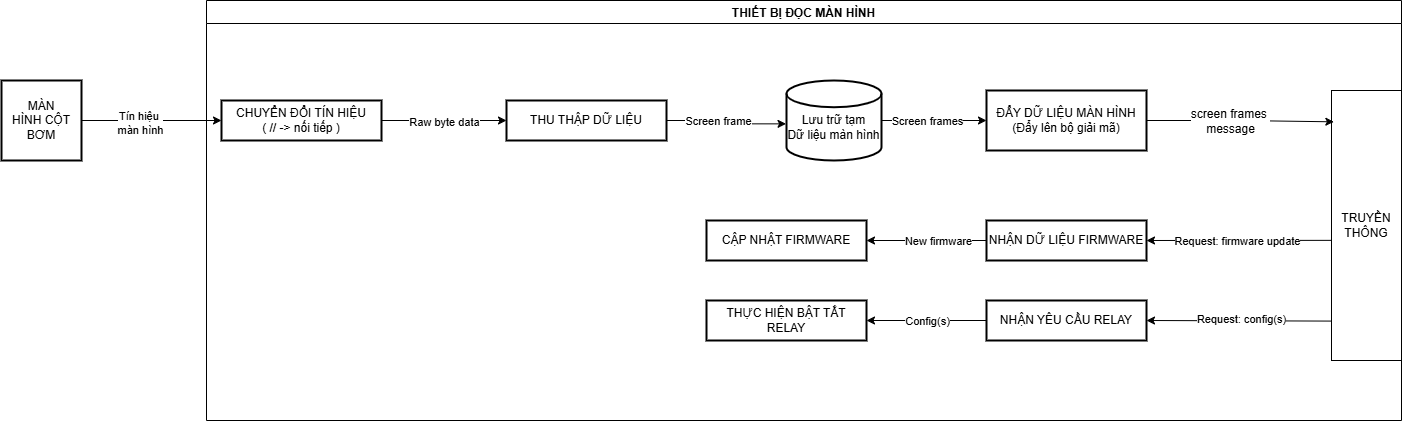
\includegraphics[width=1.0\linewidth]{Figures/Chap3_Device-FunctionBlock.png}
    \caption{Sơ đồ khối chức năng thiết bị đọc ghi màn hình (Device)}
    \label{fig:hinh3.2}
\end{figure}

\textbf{Giải thích các khối chức năng:} 

\begin{itemize}
    \item \textbf{Chuyển đối tín hiệu: }
    \subitem Nếu tín hiệu gửi tới màn hình cột bơm là nối tiếp, khối này đệm tín hiệu nối tiếp tới bộ Thu thập dữ liệu
    \subitem Nếu tín hiệu gửi tới màn hình cột bơm là song song, có nhiều chân dữ liệu, khối này chuyển đổi tín hiệu từ các chân thành tín hiệu nối tiếp -> chuyển đổi thành các SPI frame để đệm tới bộ Thu thập dữ liệu.
    \item \textbf{Thu thập dữ liệu: } Thu thập các byte data tổng hợp thành các screen frame, lưu tạm vào 1 in-mem database.
    \item \textbf{Đẩy dữ liệu lên màn hình: } Thiết bị đọc màn hình tạo 1 message (request message) gồm nhiều screen frame để đẩy lên máy tính local
    \item \textbf{Nhận và cập nhật firmware mới: } Thiết bị đọc màn hình có thể nhận firmware mới từ máy tính local hoặc Logi Service và tự động cập nhật, khởi động lại
    \item \textbf{Nhận và cập nhật relay:} Thiết bị đọc ghi màn hình có thể nhận và thực hiện yêu cầu bật tắt relay 
    \item \textbf{Truyền thông:} Lấy địa chỉ IP, dò tìm địa chỉ của phần mềm giải mã và tự động kết nối. Truyền nhận dữ liệu với phần mềm giải mã thông qua mạng LAN.

\end{itemize}

\subsubsection{Sơ đồ khối chức năng phần mềm giải mã (Device Service)}

\begin{figure}[!ht]
    \centering
    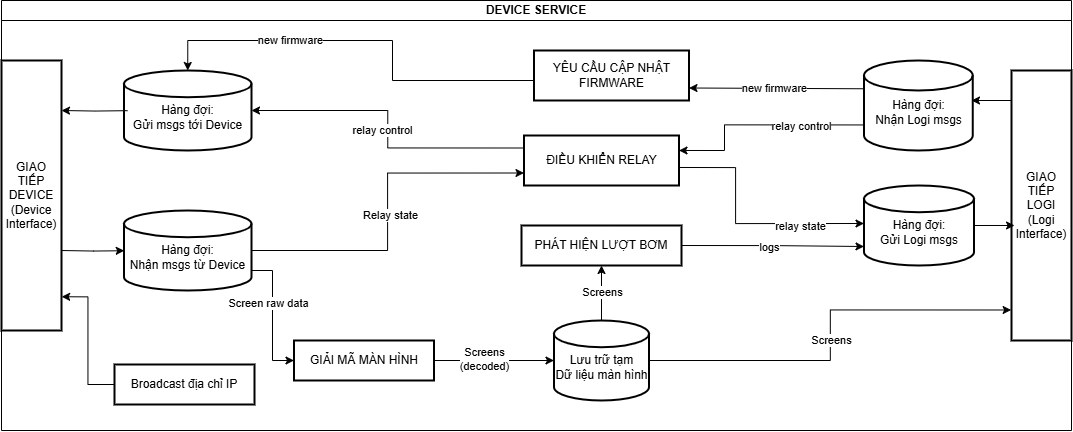
\includegraphics[width=1.0\linewidth]{Figures/Chap3_DeviceService-function-block.png}
    \caption{Sơ đồ khối chức năng phần mềm giải mã và chốt phiên bơm (Device Service)}
    \label{fig:hinh3.3}
\end{figure}

\textbf{Giải thích các khối chức năng:}

\begin{itemize}
    \item \textbf{Giao tiếp với Device (Thiết bị đọc ghi màn hình):} 
    \subitem Khối này được thiết kế chạy trên 1 luồng độc lập, nghe các yêu cầu kết nối từ thiết bị đọc ghi màn hình, kiểm tra và giữ kết nối nếu thiết bị hợp lệ 
    \subitem Truyền nhận gói tin với thiết bị đọc ghi và đẩy dữ liệu tới các khối khác để xử lý logic chính.

    \item \textbf{Giao tiếp với giao diện (GUI App):} Giữ kết nối và truyền nhận dữ liệu với phần mềm giao diện bao gồm:
    \subitem Stream dữ liệu màn hình đã giải mã theo thời gian thực.
    \subitem Gửi các phiên bơm (log) phát hiện được và trạng thái relay.
    \subitem Nhận các yêu cầu từ giao diện: cập nhật firmware, relay.
    \item \textbf{Giải mã màn hình và phát hiện phiên bơm:} Giải mã các gói tin dạng byte theo từng loại màn hình để được dữ liệu màn hình thời gian thực (số tiền, lít, đơn giá). Từ đó phát hiện trạng thái của máy (đang dừng và dừng trong bao nhiêu giây, đang tăng, reset) và phát hiện phiên bơm.
    \item \textbf{Cập nhật firmware:} Nhận file firmware từ giao diện, kiểm tra và thực hiện OTA với thiết bị đọc màn hình 
    \item \textbf{Điều khiển relay:} Chuyển tiếp gói tin yêu cầu bật tắt relay tới thiết bị đọc ghi màn hình
\end{itemize}


\subsection{Thiết kế phần cứng thiết bị đọc màn hình}

\subsubsection{Sơ đồ khối phần cứng thiết bị đọc màn hình}


\begin{figure}[!ht]
    \centering
    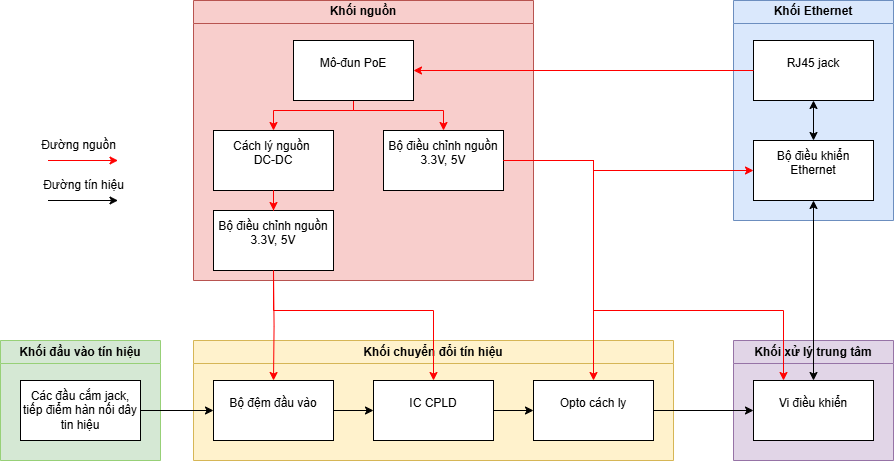
\includegraphics[width=1.0\linewidth]{Figures/Chap3_Device-Hardware-implementation-function-block.png}
    \caption{Sơ đồ khối triển khai phần cứng thiết bị đọc ghi màn hình}
    \label{fig:hinh3.4}
\end{figure}

Thiết bị mạch cứng được cấp nguồn riêng bởi POE Switch. Nguồn và tín hiệu vào được các ly bởi bộ cách ly nguồn DC-DC, các bộ đệm đầu vào và Opto cách ly, đảm bảo không ảnh hưởng tới nguồn cấp của cột bơm cũng như không có tín hiệu hay nhiễu đẩy ngược về cột bơm.

Khối đầu vào tín hiệu và khối chuyển đổi tín hiệu cũng được thiết kế thêm để thu và khảo sát được nhiều loại màn hình khác, phục vụ cho việc mở rộng chức năng hệ thống.

Thiết bị giao tiếp với phần mềm giải mã thông qua mạng LAN, sử dụng khối Ethernet.

\subsubsection{Lựa chọn linh kiện và vẽ sơ đồ nguyên lý}

\textbf{a.  Khối xử lý trung tâm}

 Yêu cầu lựa chọn:
\begin{itemize}
    \item Có 2 cổng giao tiếp SPI: mục đích để giao tiếp với khối chuyển đổi tín hiệu và với khối Ethernet. 
    \item Bộ nhớ flash lớn hơn 220KB (chứa được 2 firmware, mỗi firm ~ 110kB)
\end{itemize}

Từ những yêu cầu trên , lựa chọn STM32F407VET6 là vi điều khiển xử lý trung tâm. Các tính năng nổi bật của STM32F407VET6:

\begin{itemize}
    \item Vi điều khiển sử dụng lõi ARM Cortex-M4 32-bit, tốc độ tối đa 168 MHz, tích hợp bộ xử lý dấu chấm động (FPU) và tập lệnh DSP, phù hợp cho các ứng dụng điều khiển và xử lý tín hiệu thời gian thực.
    
    \item Bộ nhớ Flash Main Memory 512 KB, được chia thành các sector như sau:  
    
    \begin{itemize}
        \item Sector 0-3: mỗi sector 16 KB  
        \item Sector 4: 64 KB  
        \item Sector 5, 6 và 11: mỗi sector 128-KB  
    \end{itemize}

    \item Cho phép linh hoạt khi lưu nhiều firmware (ví dụ dual-bank firmware upgrade), hoặc phân vùng cho bootloader, data log, cấu hình...

    \item Tích hợp 3 cổng SPI (SPI1, SPI2, SPI3), hỗ trợ chế độ master/slave, tốc độ tối đa đến 42 MHz (SPI1) và 21 MHz (SPI2/SPI3). Phù hợp cho các giao tiếp tốc độ cao như ADC ngoại vi và module Ethernet SPI.

    \item Có tổng cộng 17 bộ Timer, gồm 12 timer 16-bit và 2 timer 32-bit. Hỗ trợ nhiều chế độ: PWM, encoder, input capture, output compare, rất hữu ích trong điều khiển động cơ, đo thời gian hoặc phát xung.

    \item Hỗ trợ nhiều chuẩn giao tiếp ngoại vi: UART, I2C, USB OTG, CAN, SDIO, Ethernet MAC - thuận tiện cho mở rộng và kết nối các module chức năng khác.

    \item Hoạt động với điện áp 1.8 V đến 3.6 V, hỗ trợ các chế độ tiết kiệm năng lượng như Sleep, Stop, và Standby - phù hợp cho ứng dụng nhúng có yêu cầu tiêu thụ điện thấp.
\end{itemize}


\begin{figure}[!ht]
    \centering
    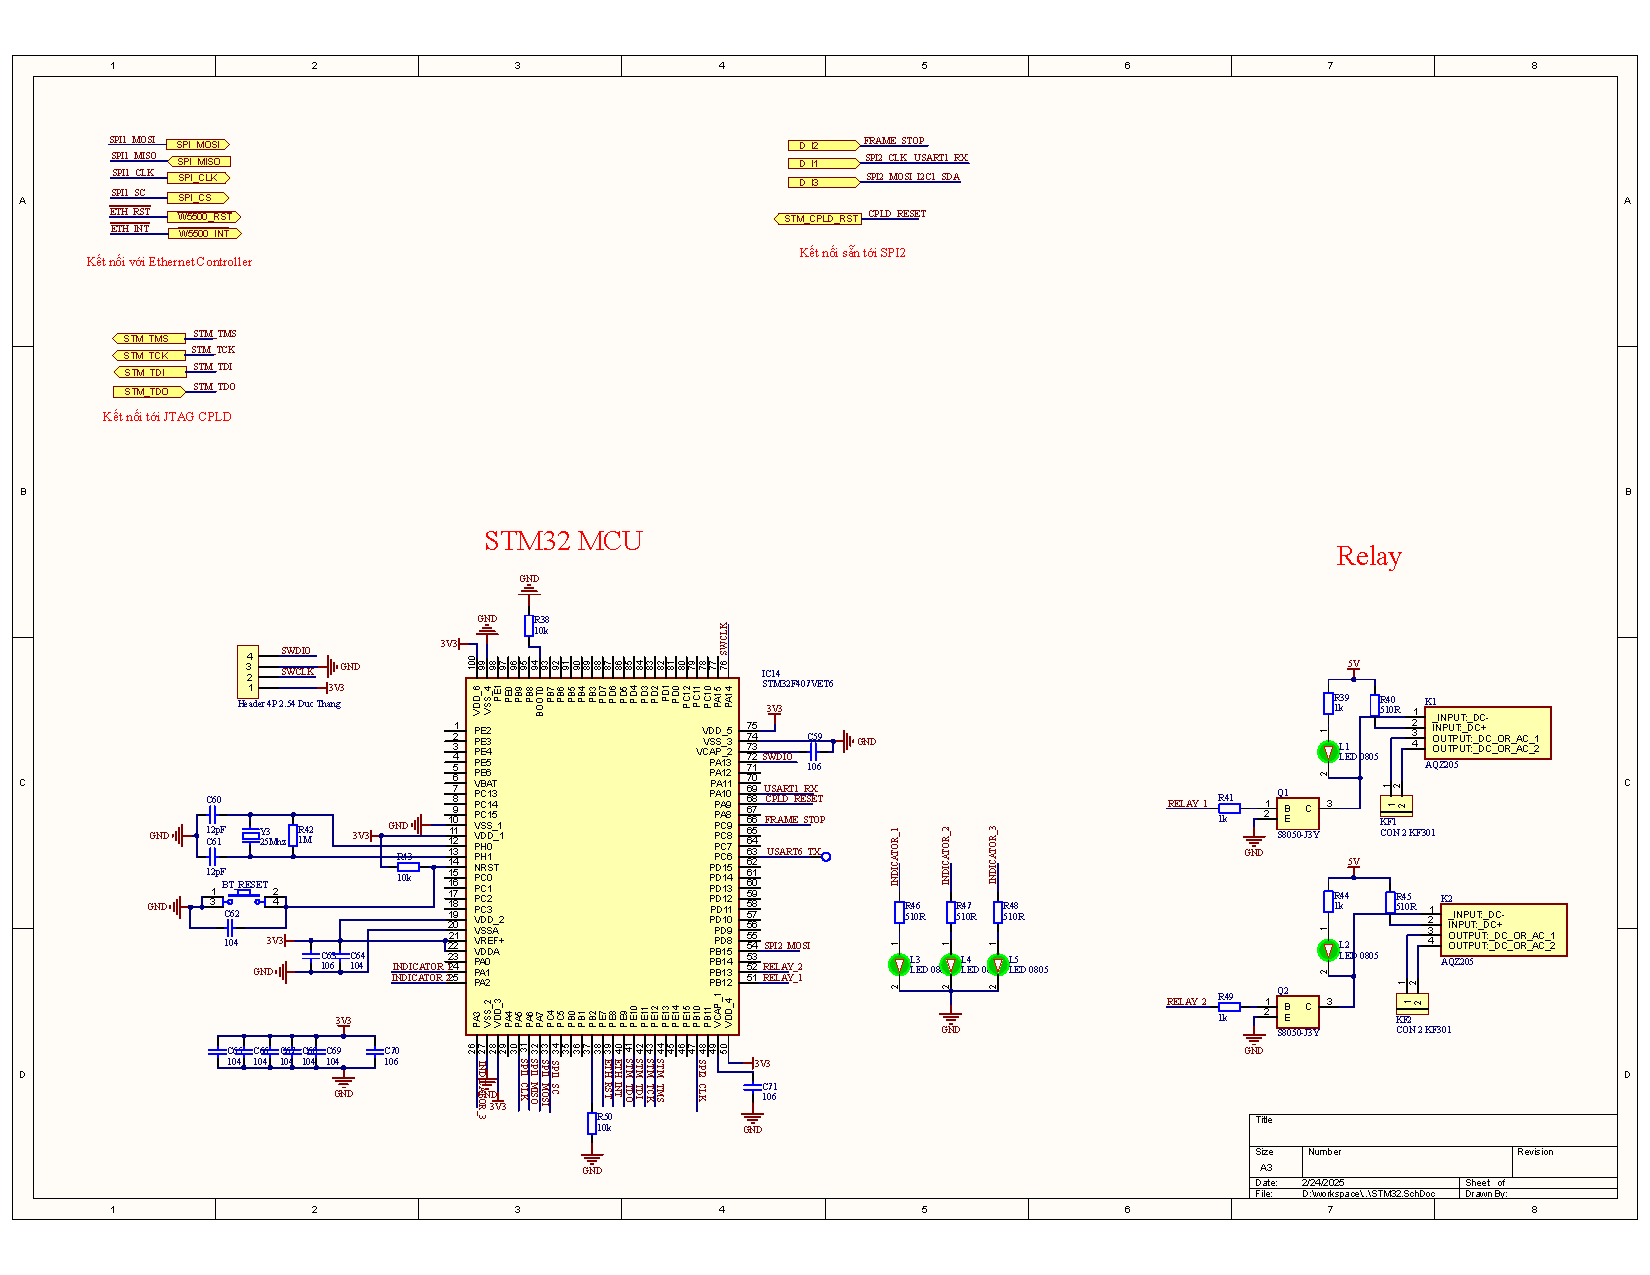
\includegraphics[width=1.0\linewidth]{Figures/Chap3_STM32-principle.pdf}
    \caption{Sơ đồ nguyên lý khối xử lý trung tâm}
    \label{fig:hinh3.5}
\end{figure}


Sơ đồ nguyên lý mạch:

\begin{itemize}
    \item Nguồn cấp 3.3V được đưa vào các chân VDD và Vref của module, các chân VSS được nối đất. Thiết kế nguồn nối với đất qua các tụ Bypass có nhiệm vụ lọc nhiễu cao tần cho nguồn nuôi vi điều khiển.
    \item Sử dụng SPI1 để giao tiếp với chip Ethernet. SPI2 để giao tiếp với khối chuyển đổi dữ liệu
    \item Các chân PA1, PA2, PA3 điều khiển đèn báo led 
    \item Reset STM32 được thực hiện khi chân NRST hạ xuống mức 0:
    \begin{itemize}
        \item Điện trở kéo lên 10K$\Omega$
        \item Tụ điện: C = 100nF, giúp tạo xung reset ngắn nhưng đủ để tái khởi STM32
    \end{itemize}
    \item Mạch nạp cho STM32:
    \begin{itemize}
        \item Thiết kế mạch nạp theo chuẩn SWD
        \item Hỗ trợ nạp thông qua mạch nạp STLink
    \end{itemize}

\end{itemize}

\textbf{Khối đầu vào tín hiệu}


 Yêu cầu lựa chọn: 

Ngoài việc thu và giải mã loại màn hình ZCheng, khối đầu vào tín hiệu còn cần hỗ trợ các loại đầu vào cho màn hình khác để thu mẫu dữ liệu, phục vụ cho việc giải mã, mở rộng hệ thống sau này. Các loại đầu vào màn hình đã khảo sát được bao gồm:

\begin{itemize}
    \item Đầu vào SPI (cho màn hình ZCheng, đã giải mã được). Loại cáp: 8P 3.96mm. Số chân tín hiệu: 3
    \item Loại cáp: 5P 3.96mm, số chân tín hiệu: 2
    \item Loại cáp: IDE 10. Số chân tín hiệu 3
    \item Loại cáp: IDE 40. Số chân tín hiệu 30
\end{itemize}

Với danh sách loại đầu vào ở trên, thiết kế khối đầu vào tín hiệu gồm các đầu jack cắm và tiếp điểm hàn để đấu nối dây điên. Khối gồm 2 phần: 

\begin{itemize}
    \item Các đầu cắm cáp: hỗ trợ các loại cáp đã khảo sát.
    \item Các điểm hàn nối dây: Trường hợp các loại màn hình khác, sẽ hàn các đường tín hiệu đó thông qua các đầu tiếp điểm hàn, kèm dây điện nối (nếu cần). Vị trí mối hàn, đấu dây sẽ cố định theo từng loại tín hiệu màn hình.
\end{itemize}

Tổng số chân cho khối đầu vào tín hiệu là 40 chân.

\begin{figure}[!ht]
    \centering
    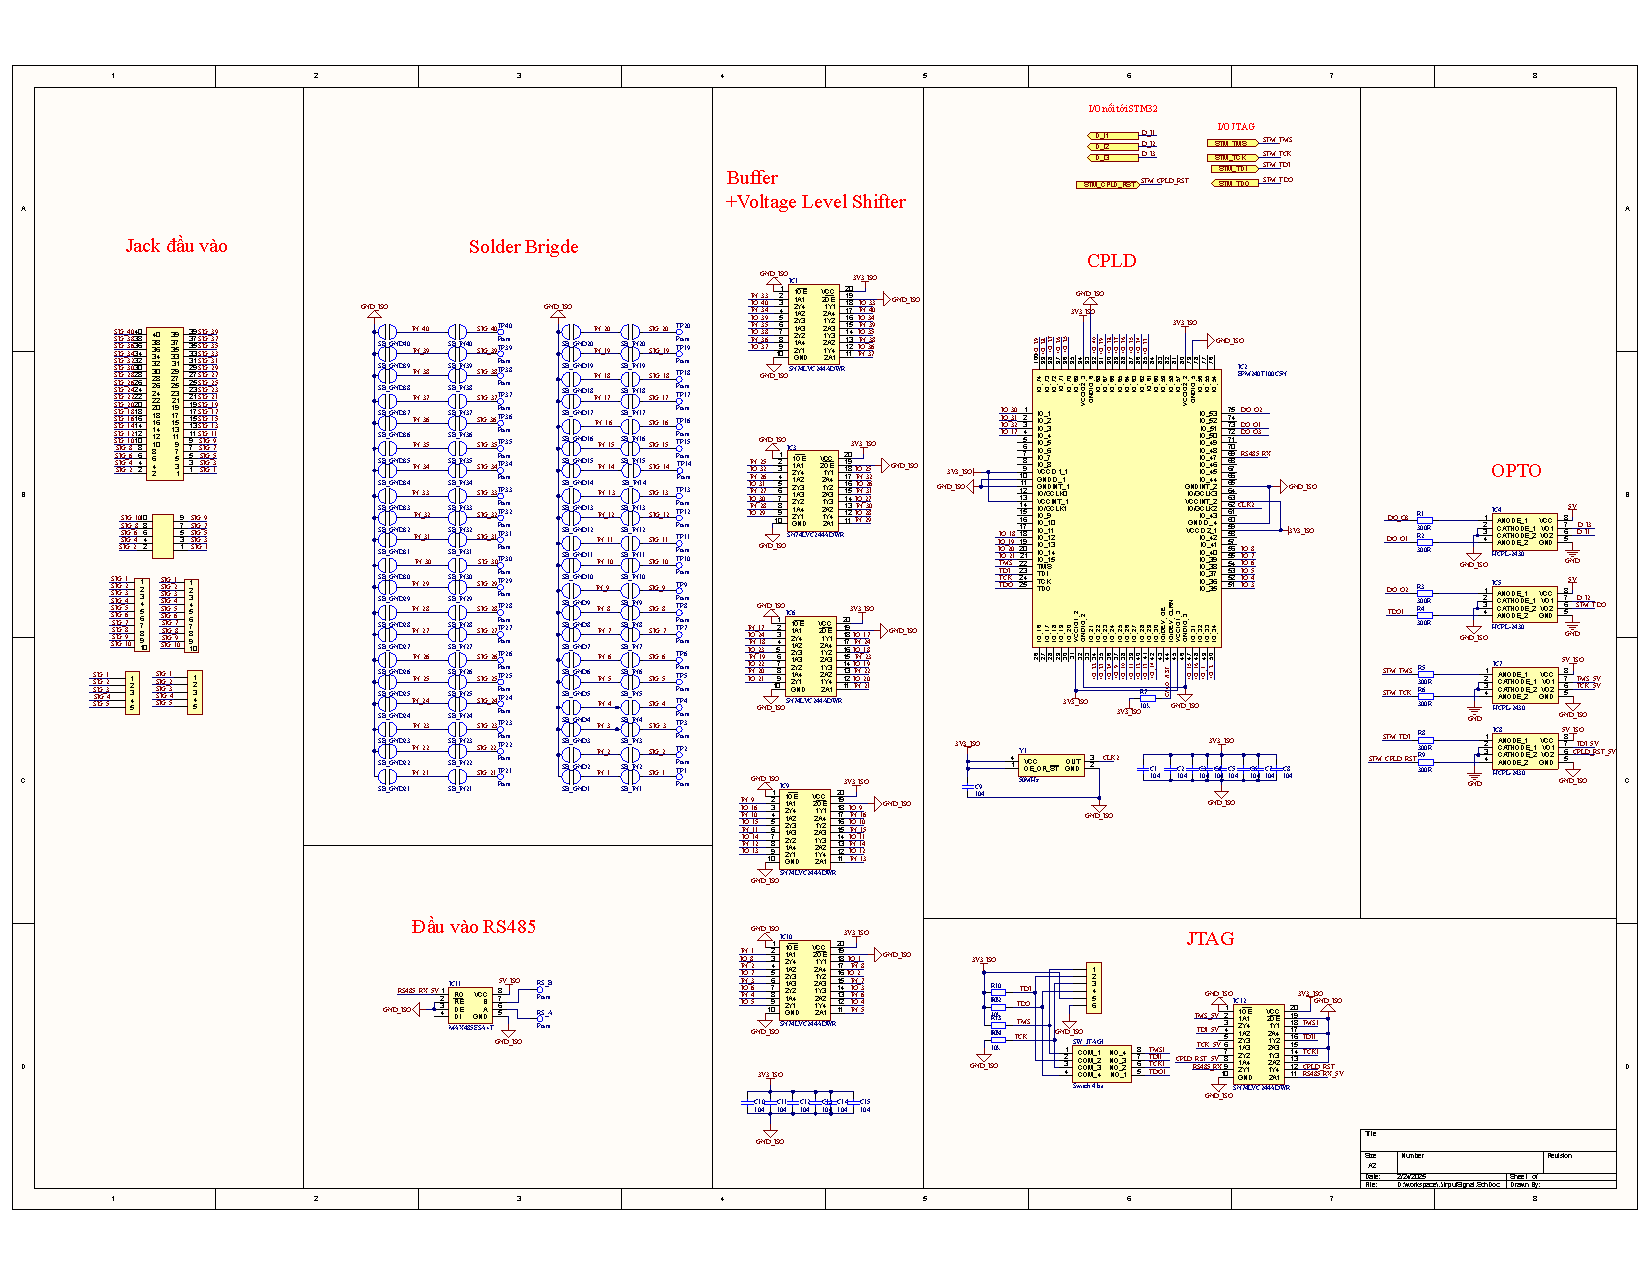
\includegraphics[width=1.0\linewidth]{Figures/Chap3_Input-signal-block-principle.pdf}
    \caption{Sơ đồ nguyên lý khối đầu vào tín hiệu}
    \label{fig:hinh3.6}
\end{figure}


\textbf{Khối nguồn và Ethernet}

Yêu cầu thiết kế: 

\begin{itemize}
    \item Khối nguồn: 
    
    \begin{itemize}
        \item Cấp nguồn 3.3V cho khối khác. Chuyển đổi nguồn 5V của POE sang 3.3V.
        \item Cách ly và chống nhiễu.
    \end{itemize}

    \item Khối Ethernet:
    \begin{itemize}
        \item Chống nhiễu.
        \item Giao tiếp với MCU (STM32) theo chuẩn SPI.
    \end{itemize}
\end{itemize}

Với những yêu cầu trên, lựa chọn:

\begin{itemize}
    \item B0505S-2WR2 và AMS1117-3.3V để cách ly và chuyển đổi nguồn POE thành nguồn 3.3V.
    \item Chip W5500 để giao tiếp Ethernet.
\end{itemize}

\begin{figure}[!ht]
    \centering
    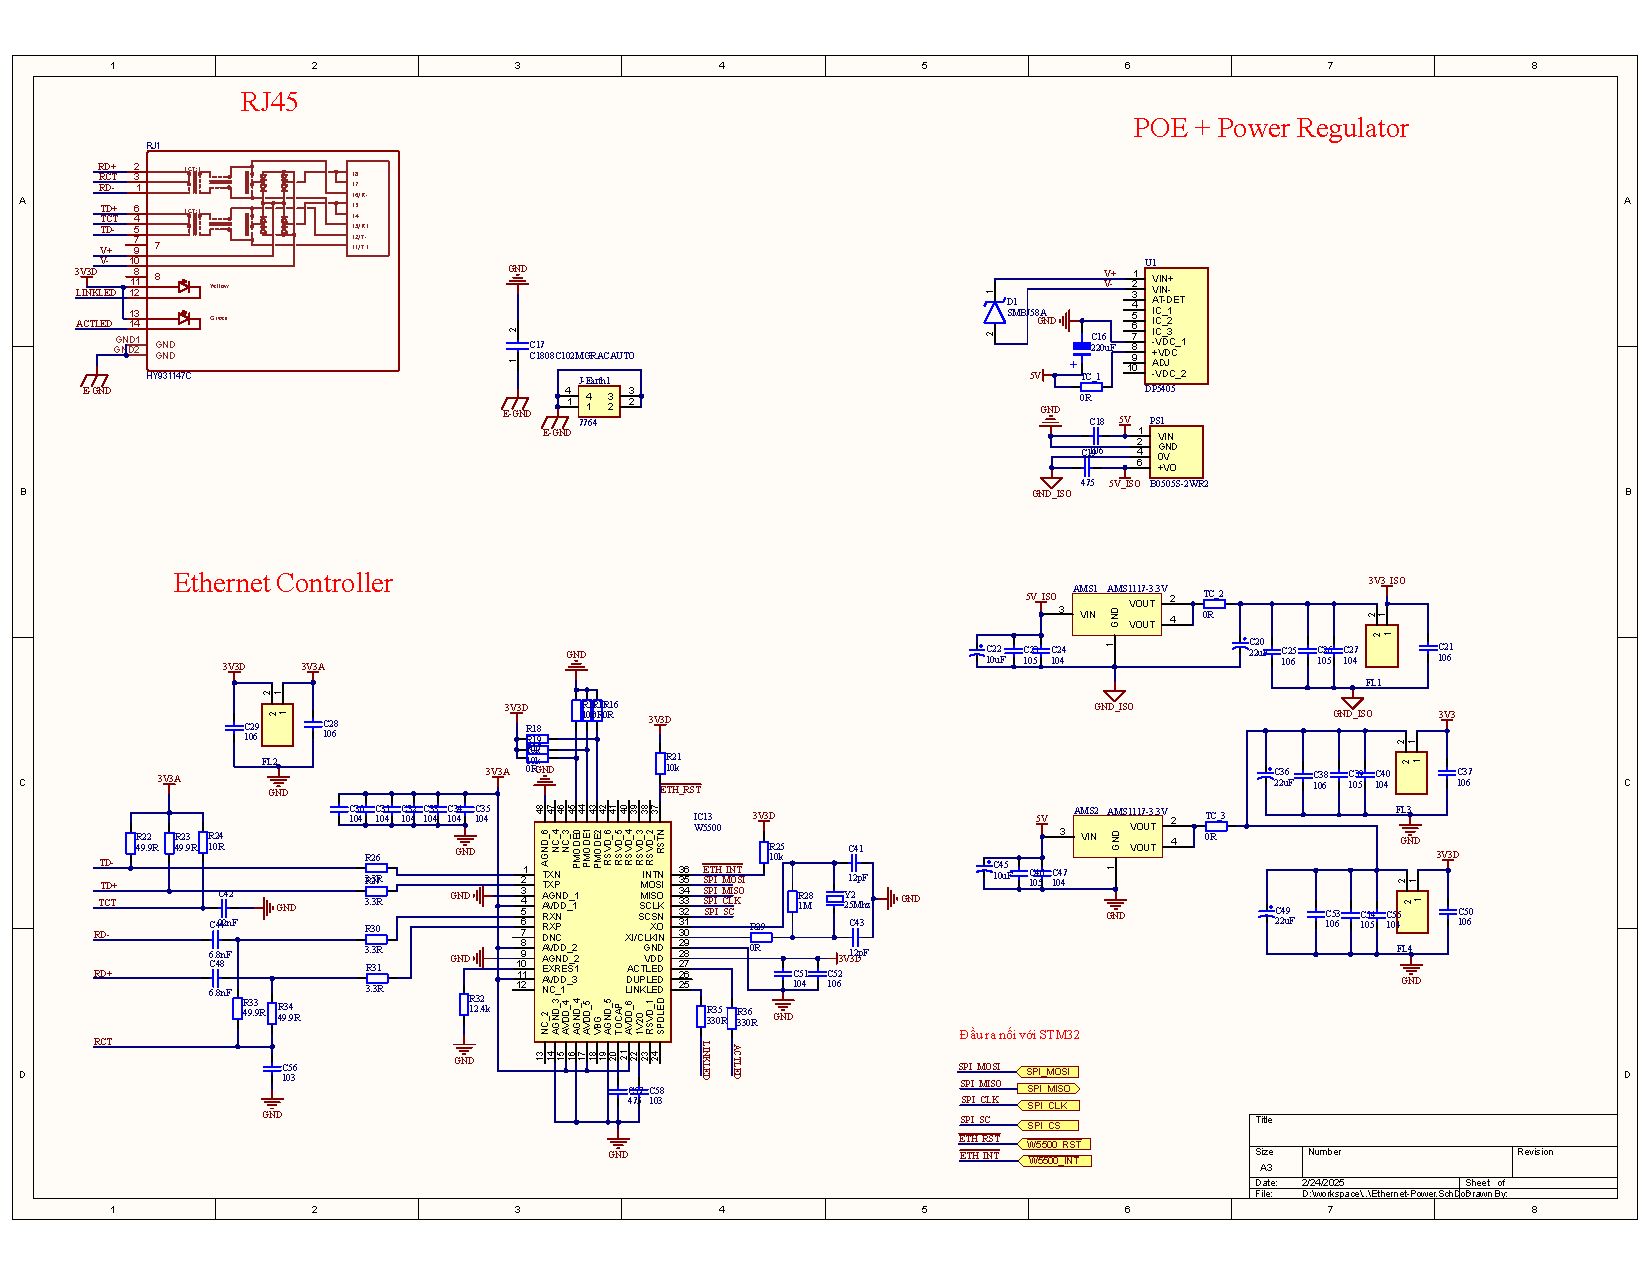
\includegraphics[width=1.0\linewidth]{Figures/Chap3_Power-and-Ethernet-block-principle.pdf}
    \caption{Sơ đồ nguyên lý khối nguồn và giao tiếp Ethernet}
    \label{fig:hinh3.7}
\end{figure}

Giải thích khối nguồn:
\begin{itemize}
    \item Mô-đun DP5405 để nhận nguồn từ PoE Switch (thông qua jack RJ45), chuyển đổi sang điện áp 5VDC để cấp nguồn cho toàn bộ thiết bị.
    
    \item IC B0505S: Có chức năng chuyển đổi điện áp 5VDC sang điện áp 5VDC cách ly. Việc cách ly nguồn để góp phần cách ly tín hiệu điện giữa tín hiệu của cáp màn hình với tín hiệu khác trong mạch, để 2 loại tín hiệu này không ảnh hưởng tới nhau.
    
    \item IC AMS1117-3.3V: Là IC điều chỉnh nguồn, đầu ra IC sẽ cung cấp nguồn điện áp 3.3V cho các linh kiện khác trong mạch. Có 2 IC trong đó IC thứ nhất để chuyển đổi điện áp 5VDC sang 3.3VDC, IC thứ hai chuyển đổi điện áp 5VDC cách ly sang 3.3V, từ đó điện áp 3.3V này cũng được cách ly với điện áp 3.3VDC ở IC thứ nhất. 
\end{itemize}

Giải thích khối Ethernet:

\begin{itemize}
    \item Jack cắm Ethernet: Sử dụng jack RJ45 HY931147C để cắm dây Ethernet vào thiết bị, vừa để dẫn nguồn cho thiết bị, vừa để hỗ trợ giao tiếp mạng Ethernet.
    \item IC điều khiển Ethernet: Sử dụng IC W5500 để cung cấp các chức năng liên quan đến truyền/nhận dữ liệu thông qua Ethernet cho khối Xử lý trung tâm.
\end{itemize}

\subsection{Thiết kế firmware thiết bị đọc màn hình}

\subsubsection {Kiến trúc triển khai firmware}

\begin{figure}[!ht]
    \centering
    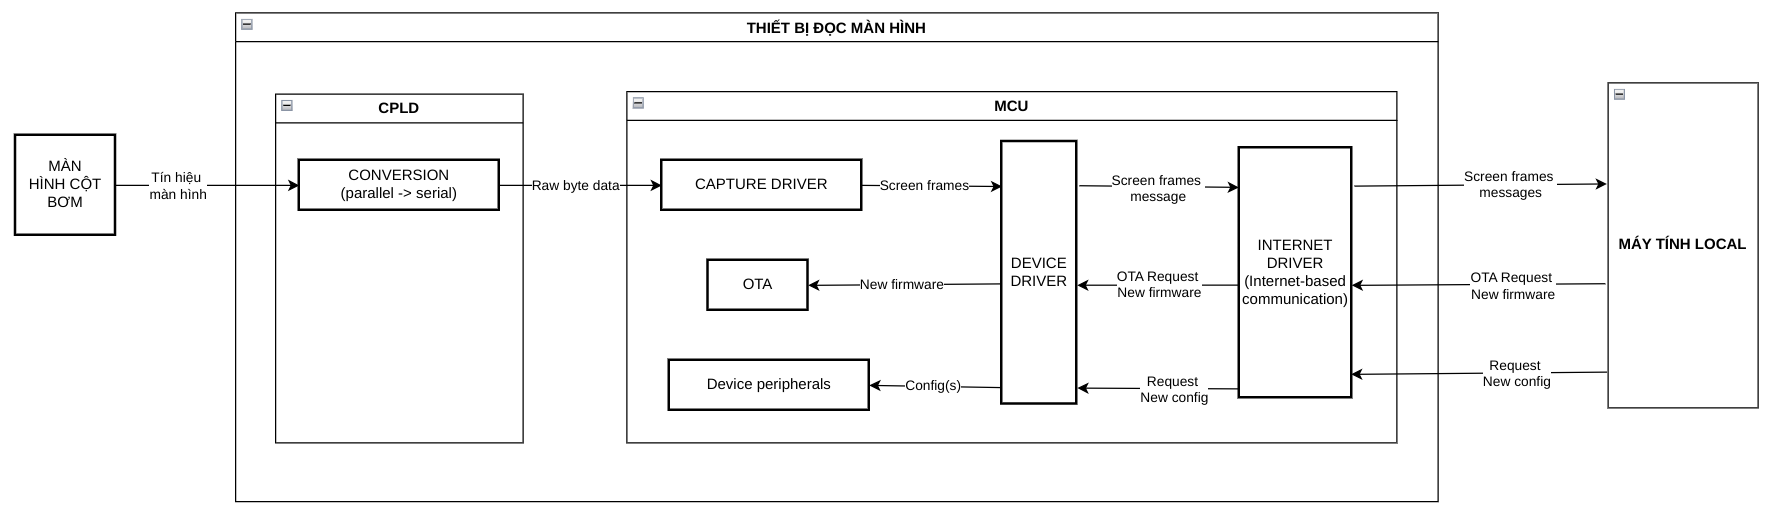
\includegraphics[width=1.0\linewidth]{Figures/Chap3_Device-block-firmware-architecture.png}
    \caption{Sơ đồ khối triển khai firmware cho thiết bị}
    \label{fig:hinh3.8}
\end{figure}

Các khối triển khai thực hiện các chức năng đã được nêu ra trong hình \ref{fig:hinh3.2}

Mỗi khối triển khai ở hình \ref{fig:hinh3.8} được tổ chức thành một module mã nguồn, xử lý và trao đổi dữ liệu với nhau.

\begin{itemize}
    \item Capture Driver: Nhận các SPI frame từ CPLD, đóng gói thành các dữ liệu màn hình dạng byte data, cùng thời gian nhận dữ liệu và loại màn hình.
    \item Device Driver: Xử lý giao thức. Xử lý các gói tin nhận được (dạng byte frame) từ đầu vào Ethernet và chuyển tiếp tới các khối Capture Driver, OTA và Device peripherals để thực hiện các logic chính. Đồng thời đẩy các gói tin màn hình (dạng byte frame) cho khối Internet để thực hiện gửi cho phần mềm máy tính (Device Service)
    \item Internet Driver: Giao tiếp với chip W5500 để thực hiện trao đổi gói tin qua mạng LAN.
    \begin{itemize}
        \item Xin cấp phát IP tĩnh từ router
        \item Nhận địa chỉ IP của phần mềm máy tính (Device Service) thông qua gói tin được broadcast
        \item Trao đổi dữ liệu dạng byte frame với phần mềm máy tính (Device Service) thông qua giao thức TCP, cấu trúc gói tin tuân theo API đã được quy ước.
        \item Khi bị mất kết nối với phần mềm Device Service, cố gắng kết nối trở lại với phần mềm.
    \end{itemize}
\end{itemize}

\subsubsection{Trình tự giao tiếp giữa các khối}

\textbf{a. Nhận gói tin broadcast và kết nối tới phần mềm Device Service}

\begin{figure}[!ht]
     \centering
    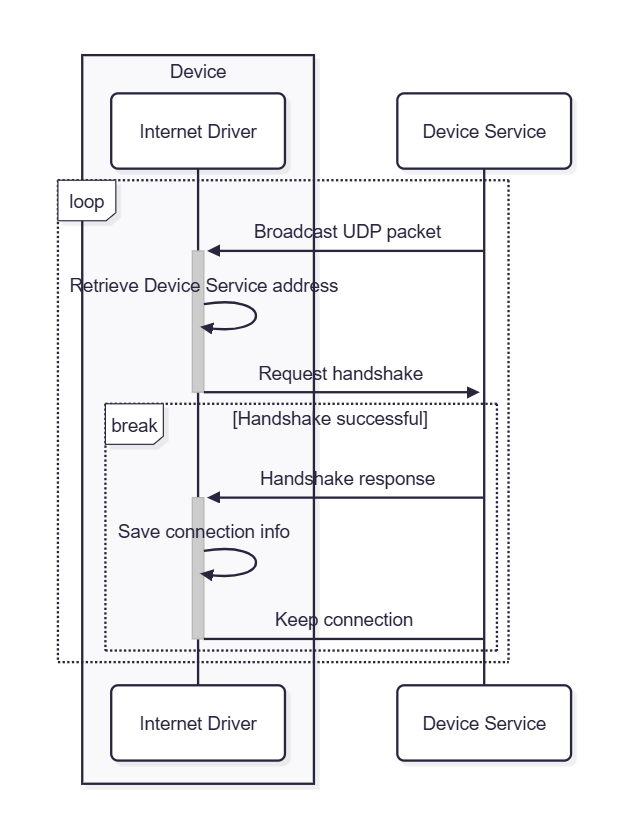
\includegraphics[width=0.8\linewidth]{Figures/Chap3_Device-firm-implementation-handshake.png}
    \caption{Trình tự giao tiếp: Thiết lập kết nối tới phần mềm giải mã Device Service}
    \label{fig:hinh3.9}
\end{figure}

Gói tin broadcast của phần mềm giải mã (Device Service) có chứa địa chỉ (IP và PORT) của phần mềm. Thiết bị nhận được gói tin, lấy thông tin địa chỉ và gửi yêu cầu thiết lập kết nối tới phần mềm (handshake).

Trong trường hợp không kết nối được hoặc mất kết nối, thiết bị sẽ liên tục yêu cầu kết nối trở lại tới phần mềm.

\textbf{b. Đẩy dữ liệu thô màn hình (dạng byte)}

\begin{figure}[!ht]
     \centering
    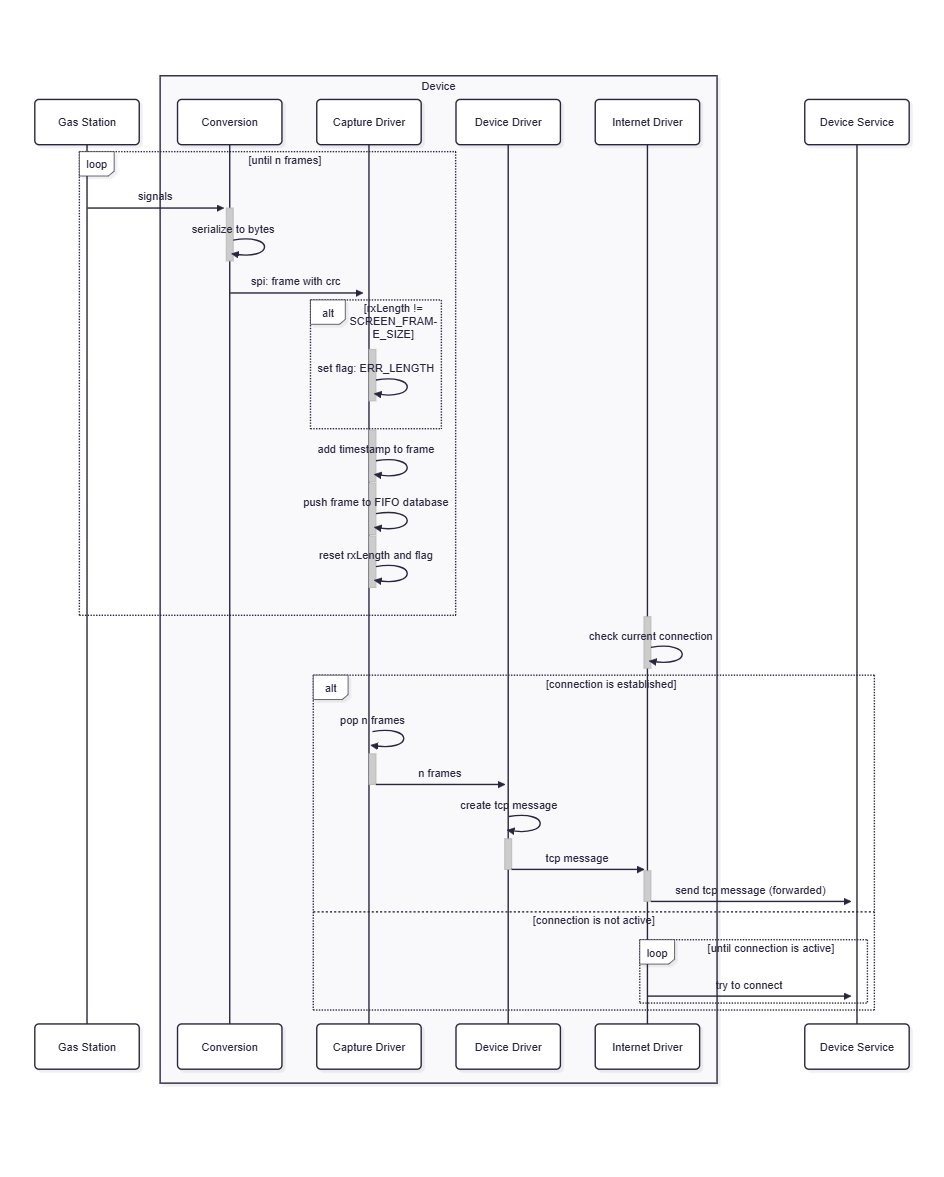
\includegraphics[width=1.0\linewidth]{Figures/Chap3_Device_firmware-implemetation-stream-screen.png}
    \caption{Trình tự giao tiếp: thu thập và đẩy dữ liệu màn hình}
    \label{fig:hinh3.10}
\end{figure}

Tín hiệu màn hình được thu thập bởi bộ chuyển đổi tín hiệu, và đẩy tới \textbf{Capture Driver}, sử dụng SPI.

Khối Capture Driver nhận từng byte, lưu trữ tạm vào 1 buffer cho đến khi độ dài buffer bằng độ dài tiêu chuẩn 1 frame màn hình (22 byte đối với máy ZCheng). Khi đó, dữ liệu buffer được lấy ra để tạo thành 1 frame màn hình.

Mỗi frame màn hình chữa dữ liệu "tổng tiền", "số lít", "đơn giá" đã được mã hóa, sẽ được lưu tạm vào 1 FIFO database (tại memory) cùng với thời gian nhận frame. Buffer nhận sau đó được xóa để bắt đầu nhận frame mới.

Do tần số nhận frame cao (100Hz), không thể gửi dữ liệu với tần số như vậy thông qua chip Ethernet, dữ liệu màn hình được lưu tạm vào 1 FIFO Database. Ở mỗi lần gửi, \textbf{Internet Driver} kiểm tra kết nối hiện tại với phần mềm Device Service. Nếu kết nối vẫn tốt, \textbf{Capture Driver} sẽ lấy nhiều frame từ database cùng một lúc để gửi đến phần mềm Device Service.

\textbf{c. Cập nhật firmware}

\begin{figure}[!ht]
     \centering
    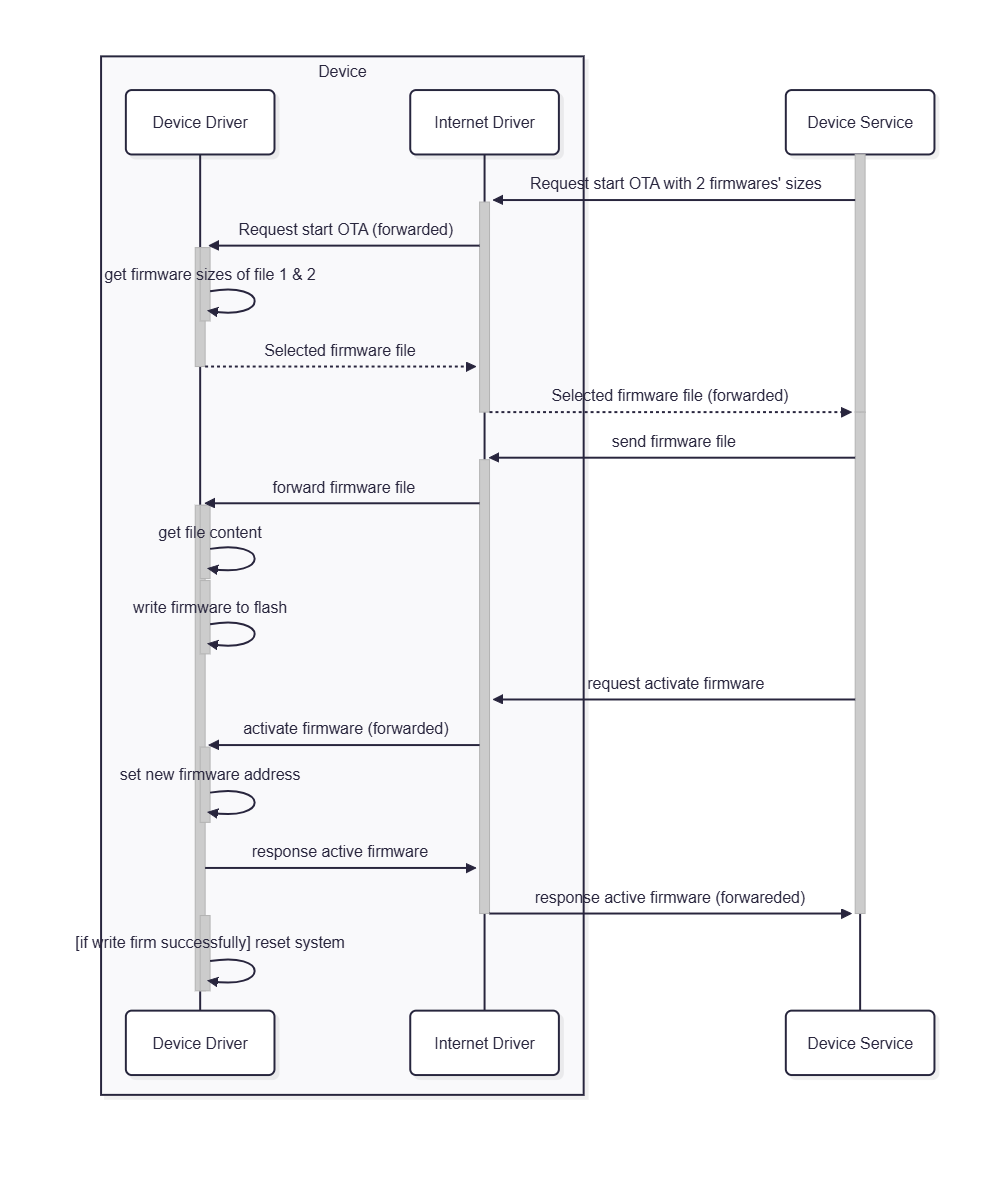
\includegraphics[width=1.0\linewidth]{Figures/Chap3_Device-firm-implementation-ota.png}
    \caption{Trình tự giao tiếp: cập nhật firmware từ xa (OTA)}
    \label{fig:hinh3.11}
\end{figure}

Phần mềm Device Service gửi yêu cầu bắt đầu tiến trình OTA cùng với kích thước firmware mới. Thiết bị thông báo lại tên file firmware muốn cập nhật (file 1 hoặc 2). 

Sau đó, Device Service gửi từng đoạn dữ liệu firmware mới cùng offset. Thiết bị dữ liệu vào flash, tại vị trí cho firmware mới.

Khi việc truyền nhận firmware mới hoàn tất, thiết bị đặt con trỏ chứa địa chỉ firmware theo giá trị địa chỉ mới và tiến hành reset.

\subsection{Thiết kế phần mềm giải mã Device Service}

\subsubsection{Kiến trúc triển khai phần mềm}

\begin{figure}[!ht]
     \centering
    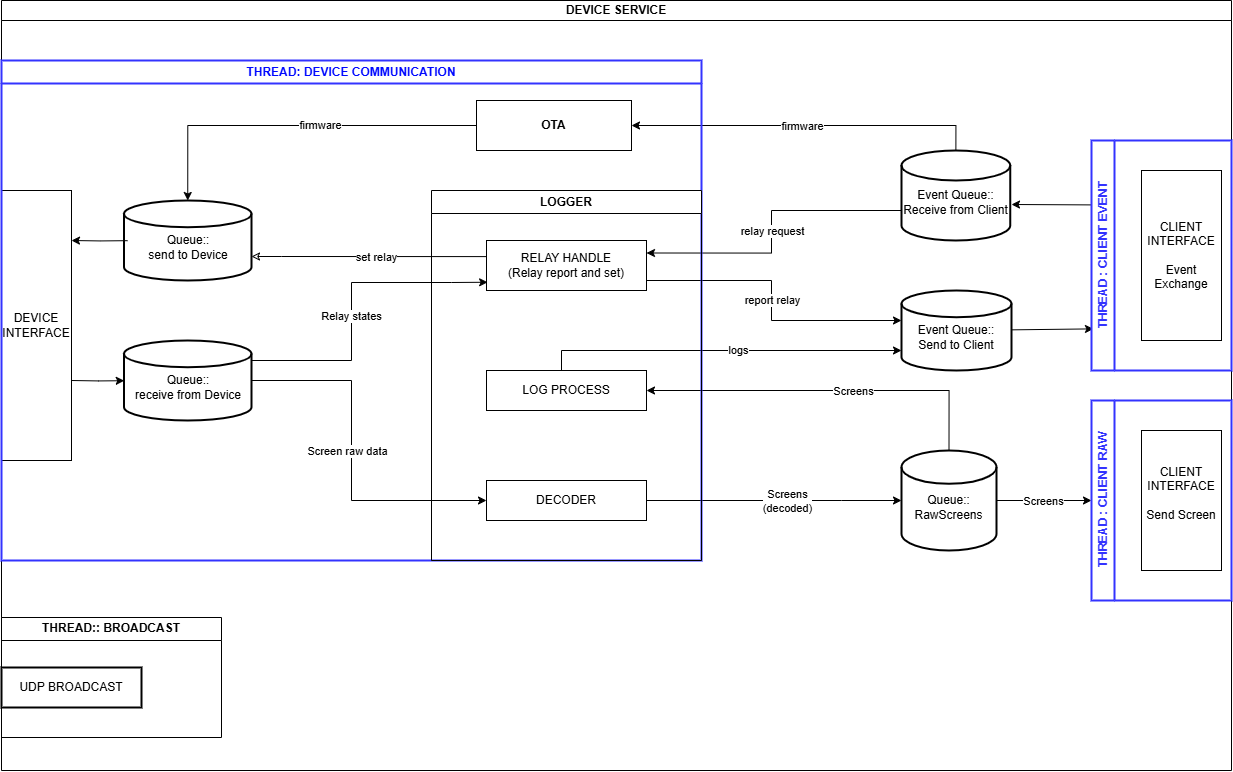
\includegraphics[width=1.0\linewidth]{Figures/DeviceService_implementation-block.png}
    \caption{Sơ đồ khối triển khai phần mềm Device Service}
    \label{fig:DeviceService_implementation-block}
\end{figure}

Các khối triển khai thực hiện các chức năng đã nêu ở
sơ đồ khối chức năng (hình \ref{fig:hinh3.3}). Về mặt triển khai, Device Service là phần mềm đa luồng, chạy dưới dạng tiến trình chạy ngầm trên máy tính nội bộ, trong đó có các luồng chính:
\begin{itemize}
    \item Device Communication giữ kết nối và giao tiếp và điều khiển thiết bị đọc ghi màn hình (Device), thực hiện giải mã và chốt phiên bơm.
    \item Client Event: luồng này trao đổi các sự kiện với phần mềm giao diện bao gồm:
    \begin{itemize}
        \item Các phiên bơm (gọi là log).
        \item Yêu cầu bật tắt relay (từ phía giao diện) và thông báo trạng thái relay (từ phía thiết bị) cho giao diện.
        \item Yêu cầu cập nhật firmware và nội dung file firmware.
    \end{itemize}

    \item Client Raw: luồng riêng biệt để gửi trực tiếp các màn hình đã giải mã theo thời gian thực, để giao diện có thể hiển thị giá trị tương ứng với màn hình cây xăng thực tế.
    
    \item Broadcast: luồng độc lập để broadcast gói tin UDP chứa địa chỉ (IP và PORT) của Device Service này cho toàn bộ thiết bị trong mạng LAN. Các thiết bị đọc ghi màn hình nhận được địa chỉ và chủ động kết nối.
\end{itemize}

Các luồng giao tiếp với nhau thông qua các hàng đợi (Queue). Các hàng đợi này được thiết kế để thread-safe, tức là các luồng chạy song song có thế truy cập vào hàng đợi mà không xảy ra xung đột.

\subsubsection{Trình tự giao tiếp và thuật toán cho các khối}

\hspace{0.8cm} Phần này trình bày trình tự giao tiếp giữa các khối trong các use case cụ thể, đồng thời trình bày các lưu đồ thuật toán quan trong. Các use case chính bao gồm:

\begin{itemize}
    \item Giải mã và gửi giá trị màn hình theo thời gian thực
    \item Cập nhật firmware cho thiết bị
    \item Gửi yêu cầu đóng ngắt relay 
\end{itemize}
\textbf{
    a. Giải mã, gửi giá trị màn hình và phát hiện phiên bơm
}

\begin{figure}[!ht]
     \centering
    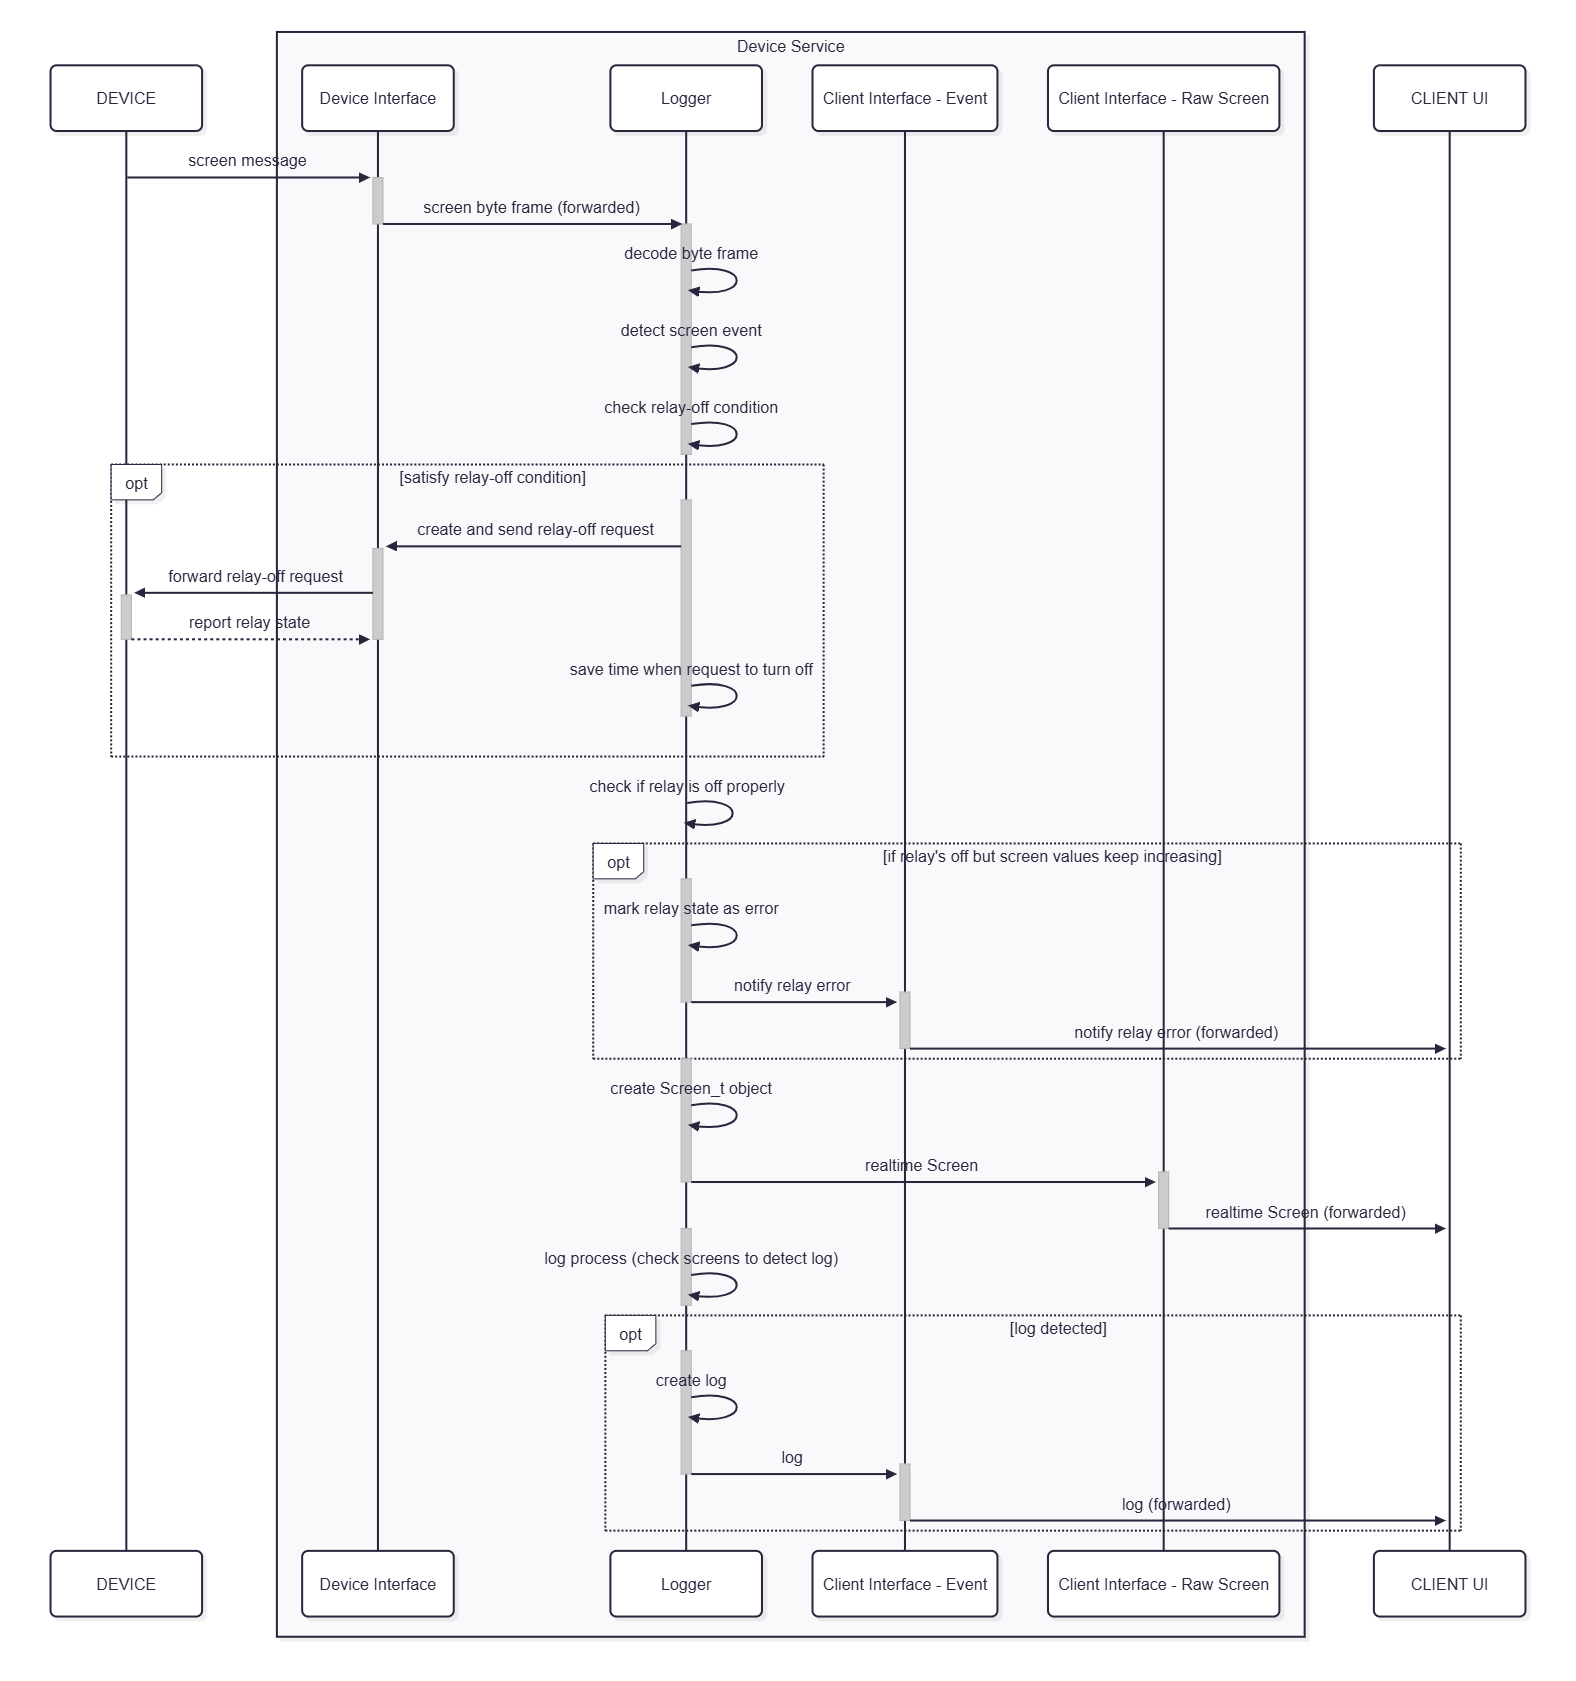
\includegraphics[width=1.0\linewidth]{Figures/DeviceService_implementation-sequence-stream-screens.png}
    \caption{Trình tự giao tiếp cho phần mềm giải mã: Giải mã màn hình}
    \label{fig:DeviceService_implementation-sequence-stream-screens}
\end{figure}

Việc giải mã tiến hành qua các bước sau:

- Giải mã dữ liệu thô dạng byte thành giá trị màn hình (số tiền, số lít, đơn giá).

- Phân loại sự kiện màn hình (screen event): 

- Phát hiện trạng thái máy (machine state).

- Phát hiện phiên bơm (log) nếu có.

Dữ liệu thô từ màn hình cây xăng được đọc liên tục, decode và so sánh để xác định giá trị và độ biến thiên giá trị đang hiển thị ở cột bơm (`bằng 0 | đang tăng | đang dừng`), xác định trạng thái hiện tại của cột bơm (`reset | đang bơm | tạm dừng bơm`). Từ đó đưa ra quyết định chốt một lượt bơm - gọi là 1 `log`.






\textbf{
b. Điều khiển relay cho thiết bị 
}

Từ giao diện người dùng Client UI, có thể:

\begin{itemize}
    \item Gửi yêu cầu bật tắt relay. 
    \item Đặt ngưỡng giới hạn trên (số tiền hoặc số lít) để relay tự động tắt.
\end{itemize}


\begin{figure}[!ht]
     \centering
    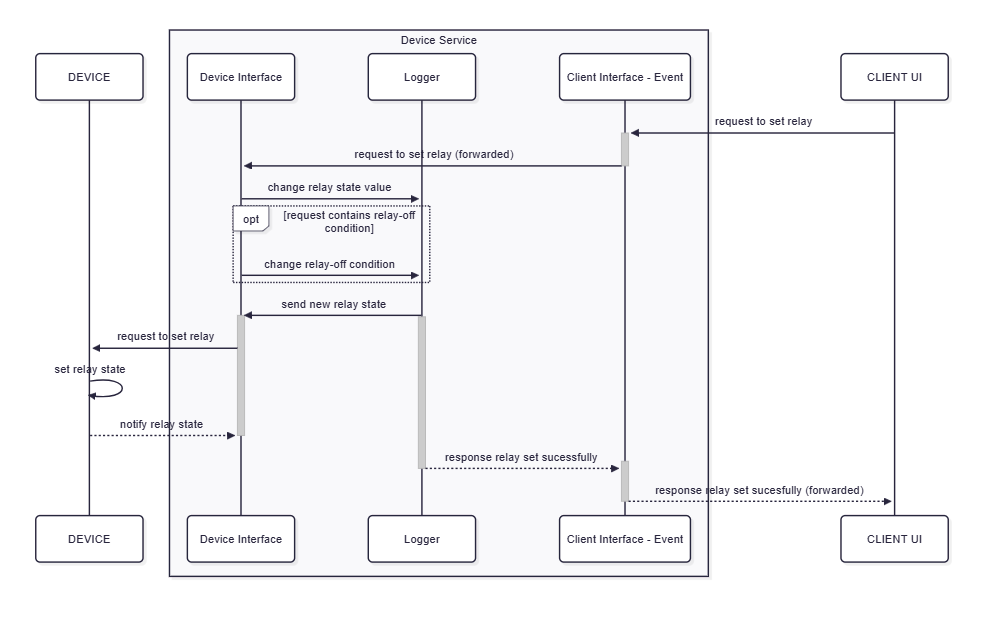
\includegraphics[width=0.8\linewidth]{Figures/DeviceService_implemetation-sequece-relay-control.png}
    \caption{Trình tự giao tiếp phần mềm trong trường hợp điều khiển relay}
    \label{fig:DeviceService_implemetation-sequece-relay-control}
\end{figure}

\FloatBarrier

\textbf{
c. Cập nhật firmware từ xa (OTA) 
}

File firmware mới được gửi từ Client UI, được mã hóa dưới dạng base64 string. Phần mềm Device Service giải mã và kiểm tra hợp lệ (verify hash) rồi lưu tạm vào RAM. Sau khi nhận được yêu cầu kích hoạt quá trình OTA, Device Service bắt đầu gửi từng đoạn firmware mới tới thiết bị đọc ghi màn hình.

\begin{figure}[!ht]
     \centering
    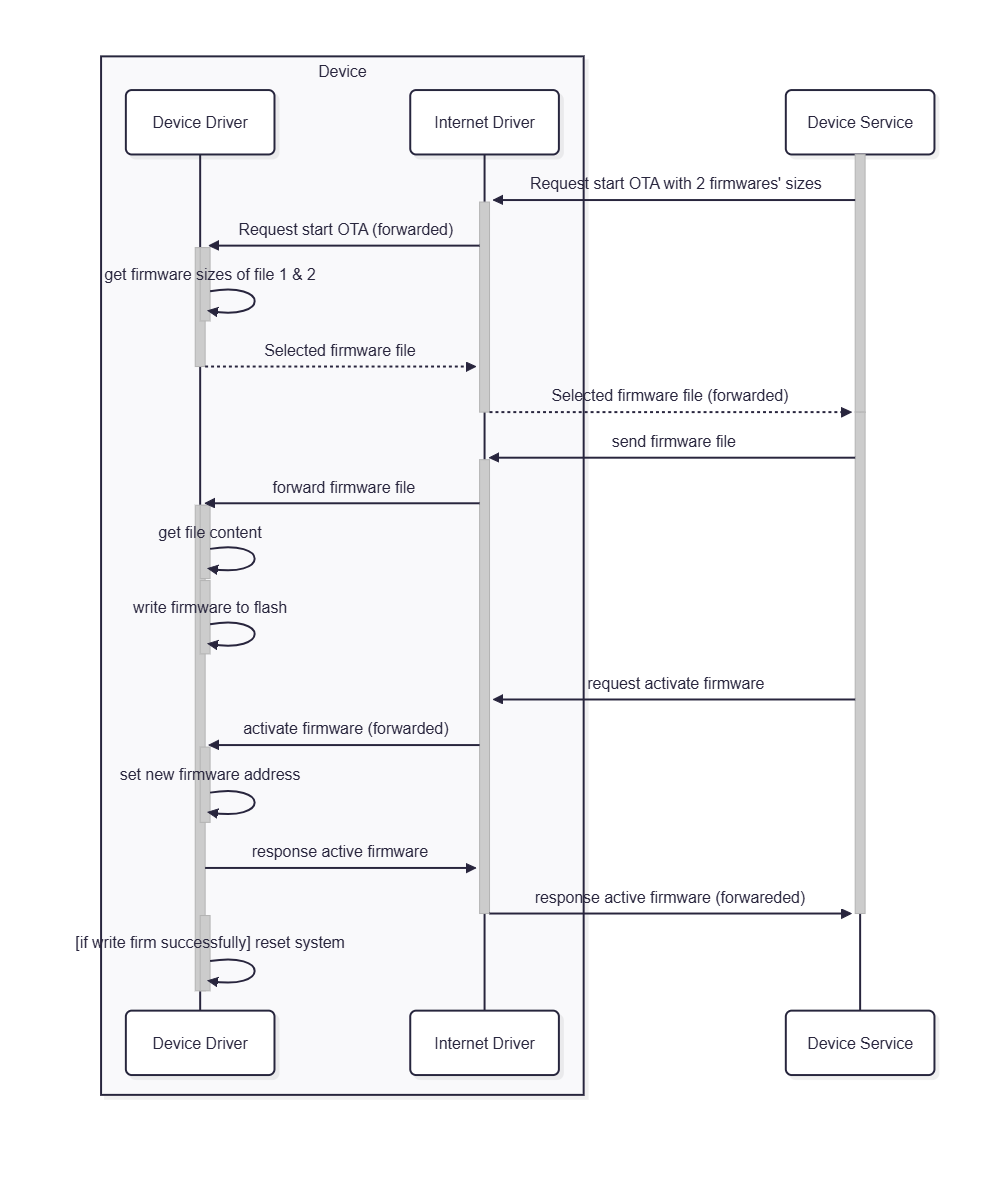
\includegraphics[width=0.8\linewidth]{Figures/Chap3_Device-firm-implementation-ota.png}
    \caption{Trình tự giao tiếp phần mềm trong trường hợp thực hiện OTA}
    \label{fig:Chap3_Device-firm-implementation-ota}
\end{figure}

\FloatBarrier

\subsection{Giao diện điều khiển cho người dùng}

\hspace{0.8cm} Phần mềm giao diện được thiết kế cho người dùng cuối để lưu trữ, hiển thị và điều khiển phần mềm giải mã Device Service.

Yêu cầu thiết kế:

\begin{itemize}
    \item Giao diện trực quan, gần gũi với người dùng.
    \item Độc lập với Device Service, kiến trúc có thể dễ dàng mở rộng, hướng tới trở thành công cụ trực quan có thể quan sát và hỗ trợ debug cho Device Service.
    \item Tương tác với cơ sở dữ liệu để đọc ghi các phiên bơm.
\end{itemize}

\begin{figure}[!ht]
     \centering
    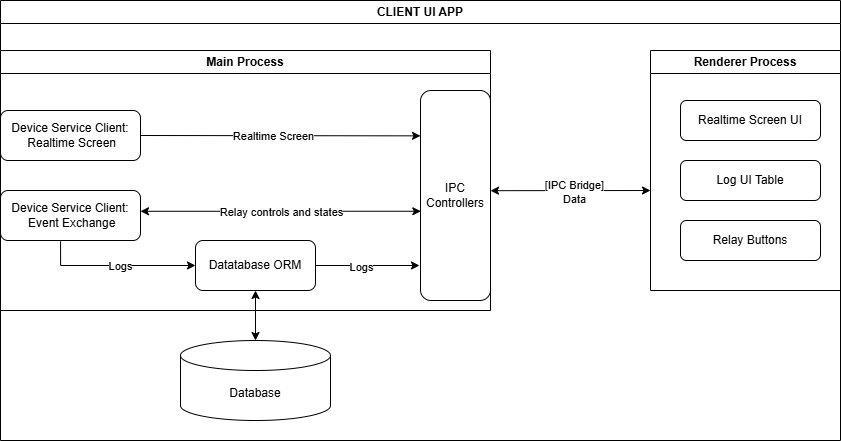
\includegraphics[width=0.8\linewidth]{Figures/ClientUI_implementation-block.png}
    \caption{Sơ đồ khối triển khai phần mềm giao diện}
    \label{fig:ClientUI_implementation-block}
\end{figure}

Phần mềm giao diện xây dựng trên môi trường Nodejs, sử dụng framework Electron để tạo một web-based Desktop App. Phần mềm gồm 2 tiến trình (process) chính:

\begin{itemize}
    \item Main Process có thể tương tác trực tiếp với hệ điều hành thông qua môi trường NodeJS. Sử dụng để:
    \begin{itemize}
        \item Mở các cổng TCP hứng dữ liệu (màn hình thời gian thực, các events) từ phần mềm giải mã Device Service.
        \item Xử lý các logic, tương tác với cơ sở dữ liệu: đọc và ghi các phiên bơm (log).
        \item Chuyển tiếp các dữ liệu lên phía Renderer Process để hiển thị lên giao diện
    \end{itemize}

    \item Renderer Process là tiến trình sử dụng để hiển thị giao diện, tương tác với người dùng. Tiến trình này bản chất là 1 module có lõi là Chromium. Bản chất của việc render và hiển thị  sử dụng các công nghệ web broswer (HTML, CSS, JavaScript) để vẽ các element. Do đó, việc tương tác trực tiếp với hệ điều hành cũng bị hạn chế, cần có Main Process và IPC (InterProcess Communication) để người dùng thực hiện các tác vụ với hệ điều hành và cơ sở dữ liệu thông qua giao diện.
    
\end{itemize}

Phần mềm có một cơ chế IPC (InterProcess Communication) riêng để các process giao tiếp với nhau, giúp chia sẻ dữ liệu an toàn.
\begin{figure}[!ht]
     \centering
    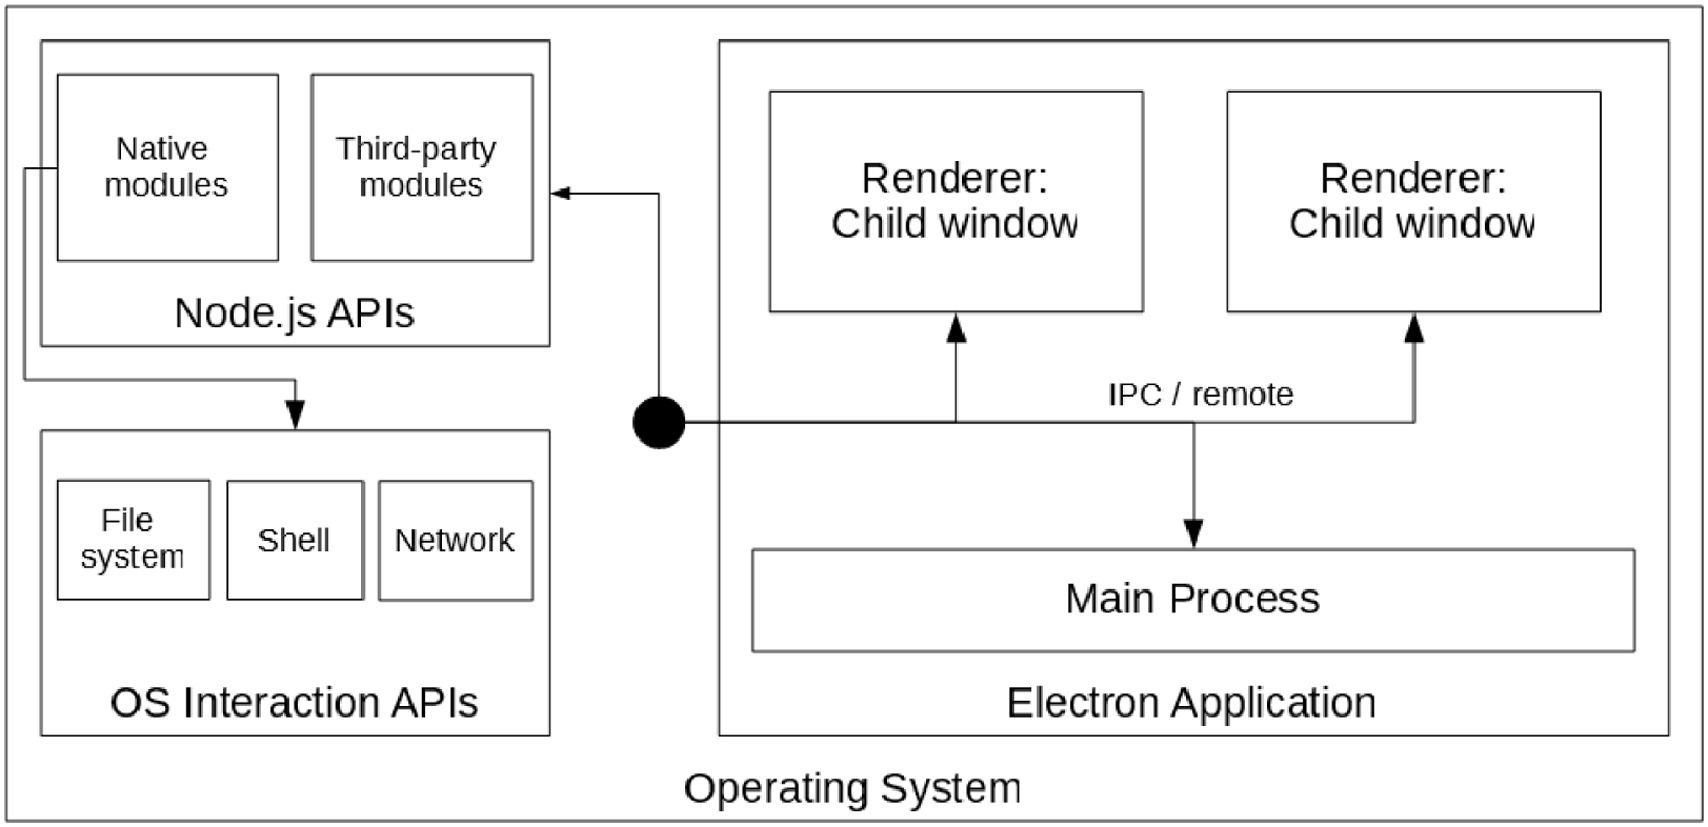
\includegraphics[width=0.8\linewidth]{Figures/Electron_IPC_mechanism.jpg}
    \caption{Giao tiếp giữa các process của ứng dụng thông qua IPC}
    \label{fig:Electron_IPC_mechanism}
\end{figure}

\FloatBarrier
\subsection{Tổng kết chương}

Trong chương này đã trình bày các khối chức năng của các thành phần hệ thống. Từ yêu cầu về chức năng đó, đưa ra thiết kế chi tiết bao gồm:

\begin{itemize}
    \item Sơ đồ nguyên lý mạch cứng 
    \item Sơ đồ triển khai phần mềm
    \item Tương tác giữa các khối trong phần mềm.
\end{itemize}

Và diễn giải các sơ đồ.


















